\chapter{Računalni vid u prepoznavanju penjačkog smjera}

Prepoznavanje specifičnih objekata sa slike, u ovom slučaju prepoznavanje penjačkih smjerova na slici stijene, zahtijeva primjenu metoda koje su otporne na promjene u osvjetljenju, udaljenosti i kutu gledanja. Pristupi koji se temelje na uspoređivanju piksela slike su neefikasni i nepouzdani jer su osjetljivi na spomenute varijacije. Zbog toga se koriste robusnije metode temeljene na detekciji i opisu lokalnih značajki (eng. \textit{feature-based methods}). Temeljna ideja je pronaći jedinstvene, stabilne i ponovljive točke na slici, značajke, te ih iskoristiti za usporedbu i prepoznavanje.

Cjelokupni proces prepoznavanja penjačkog smjera pomoću detekcije značajki zahtijeva tri komponente, referentnu sliku penjačkog smjera, referentnu sliku linije penjačkog smjera te sliku stijene dobivene s kamere mobilnog uređaja (slika~\ref{fig:tri_kljucne_slike}).

\begin{figure}[H]
    \centering
    \begin{subfigure}[b]{0.32\textwidth}
        \centering
        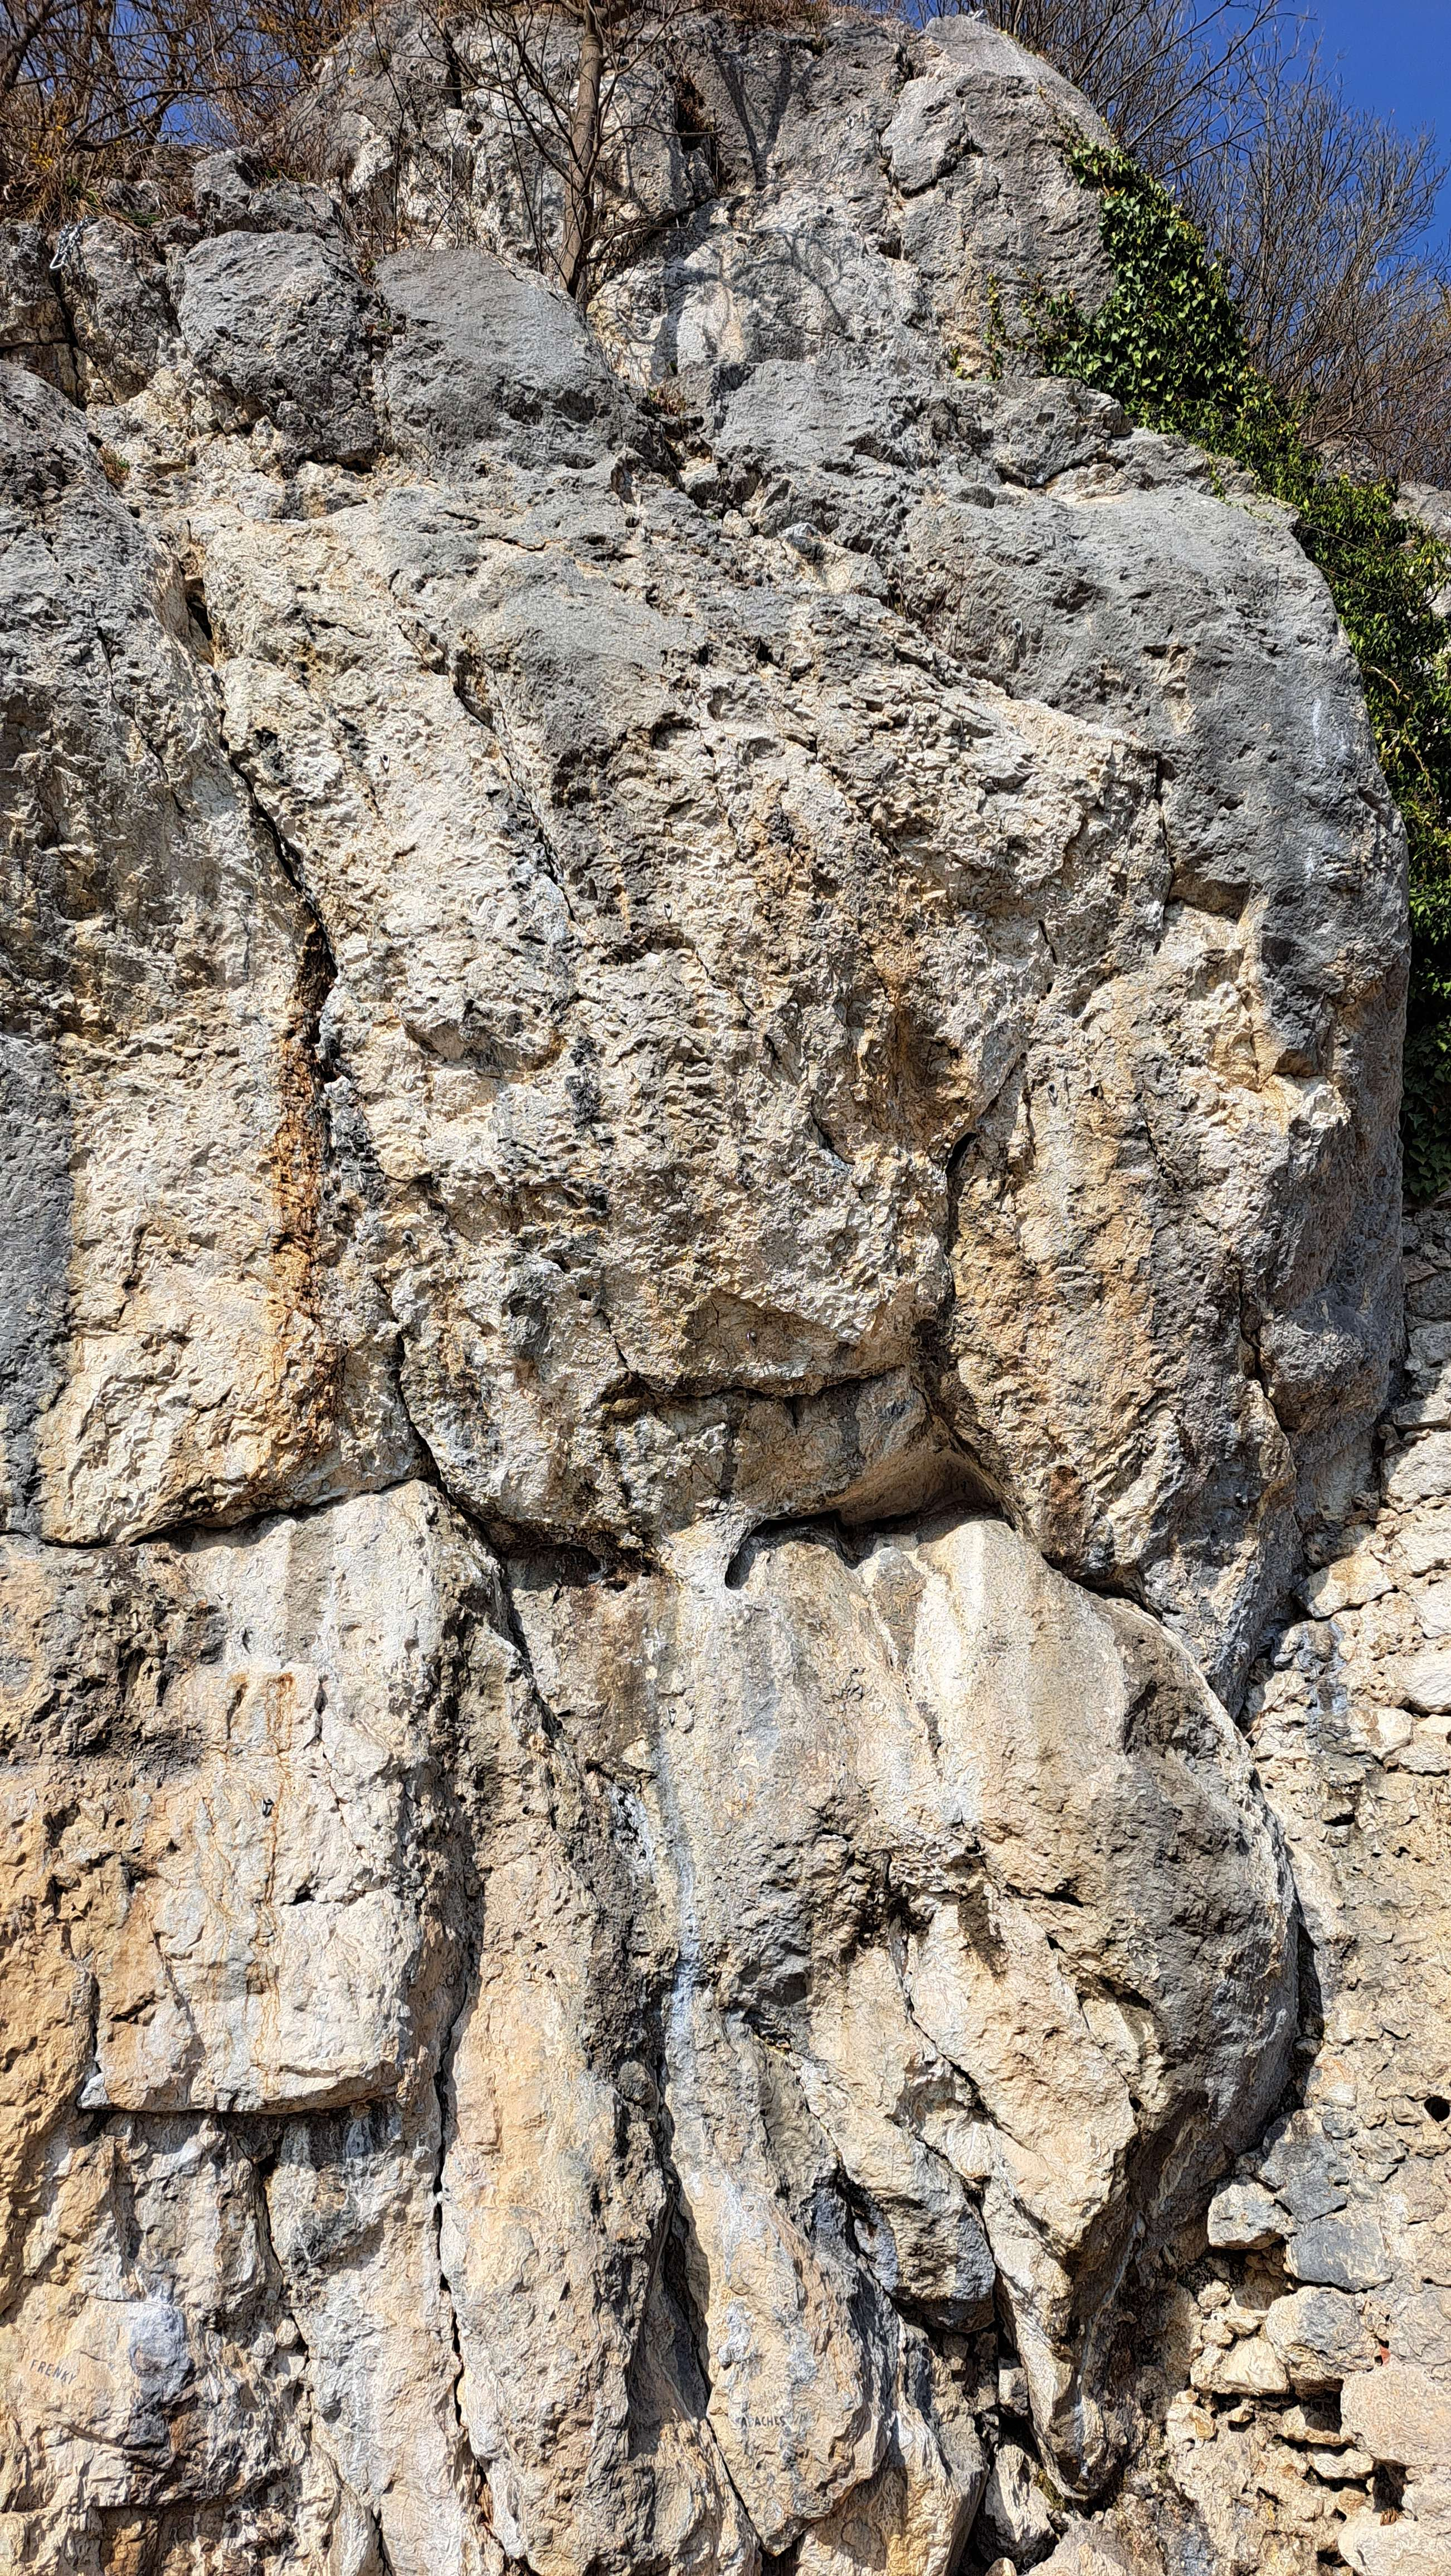
\includegraphics[width=\textwidth]{images/racunalniVid/apaches_frame.jpg}
        \caption{Slika stijene dobivena s kamere}
        \label{fig:referentna_slika_stijene}
    \end{subfigure}
    \hfill
    \begin{subfigure}[b]{0.32\textwidth}
        \centering
        \includegraphics[width=\textwidth]{images/racunalniVid/apaches_ref_photo.png}
        \caption{Referentna slika stijene}
        \label{fig:referentna_slika_linije}
    \end{subfigure}
    \hfill
    \begin{subfigure}[b]{0.32\textwidth}
        \centering
        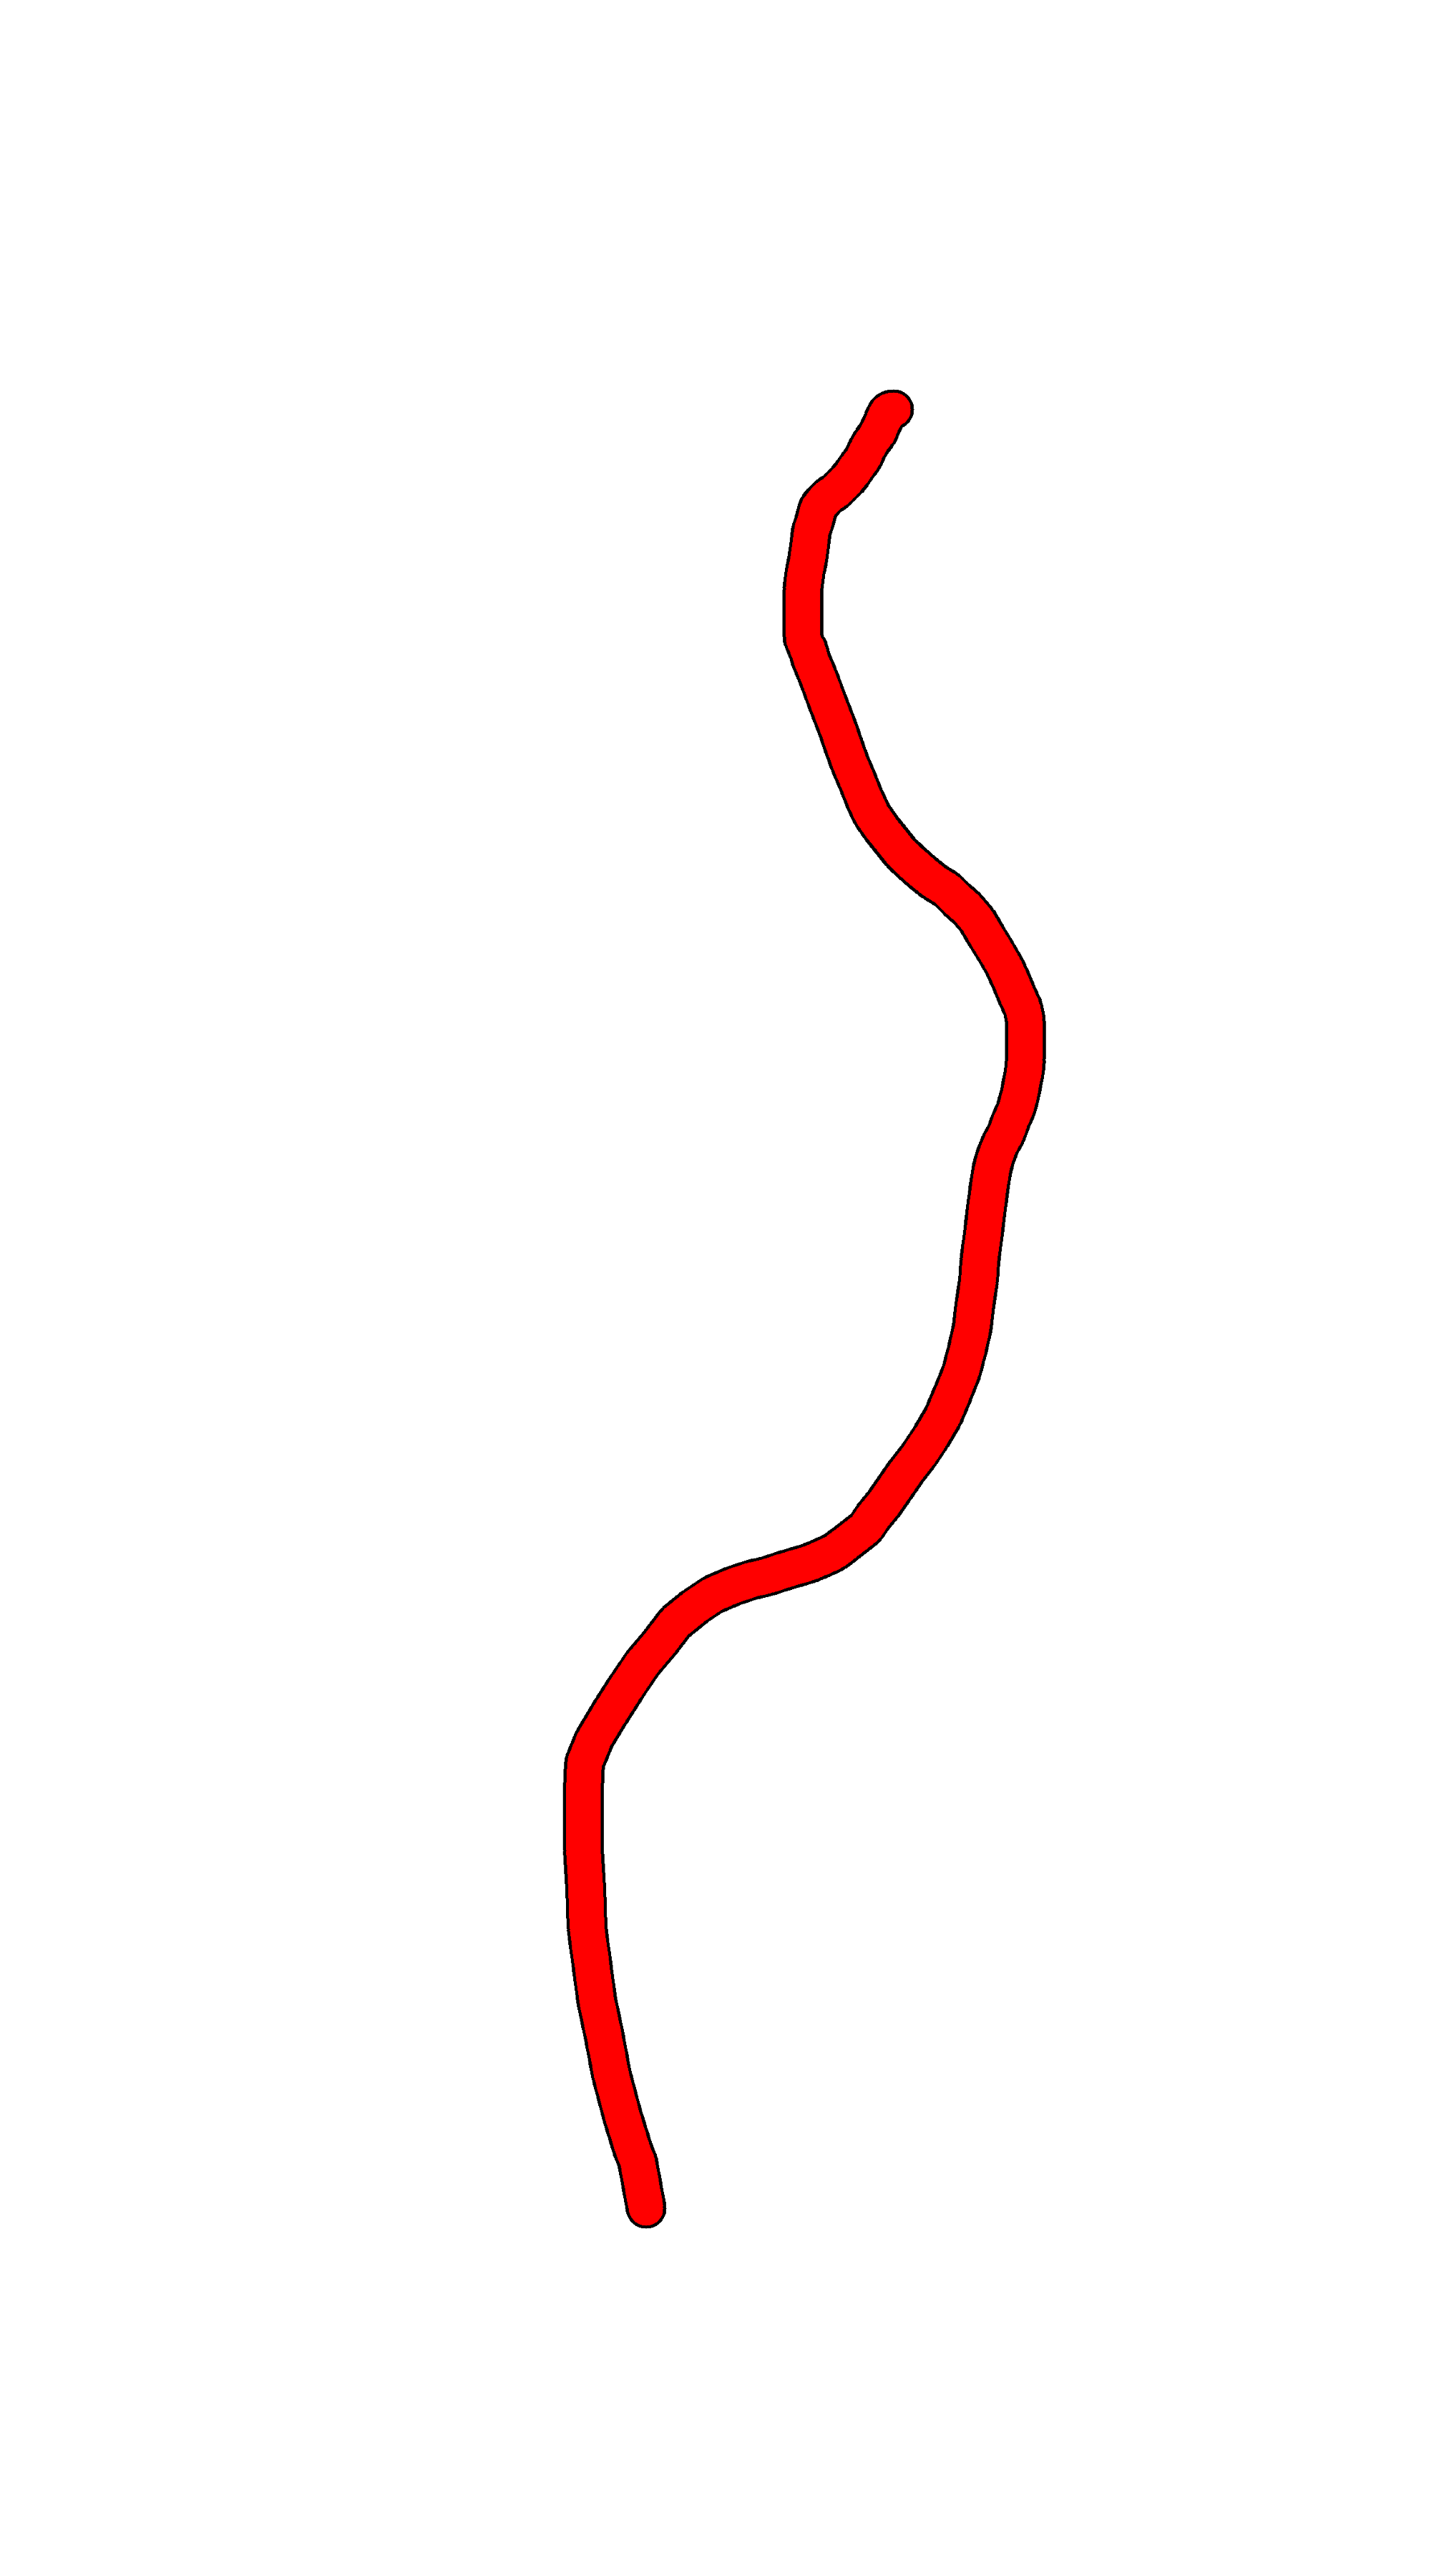
\includegraphics[width=\textwidth]{images/racunalniVid/apaches_line.png}
        \caption{Referentna slika linije smjera}
        \label{fig:slika_stijene_kamera}
    \end{subfigure}
    \caption{Tri slike potrebne za prepoznavanje penjačkog smjera}
    \label{fig:tri_kljucne_slike}
\end{figure}

Referentna slika penjačkog smjera te referentna slika linije penjačkog smjera moraju biti iste dimenzije. Proces se može se raščlaniti na sljedeće korake.
Prvi korak je detekcija i opis značajki, gdje se na referentnoj slici, unaprijed pripremljenoj slici stijene, i slici dobivenoj s kamere pronalaze ključne točke te se za svaku ključnu točku generira jedistveni numerički opis, odnosno deskriptor. Potom se uparuju značajke između slika uspoređujući deskriptore, tipično koristeći algoritam poput \textit{FLANN Matcher}. 
Te uparene značajke koriste se u trećem koraku, gdje se računa procjena geometrijske transformacije. Računa se matematički model - homografija, koja opisuje kako je slika stijene dobivene s kamera rotirana, skalirana i perspektivno izobličena u odnosu na referentnu sliku. Konačno provodi se primjena transformacije, gdje se izračunati model koristi kako bi se referentna slika linije penjačkog smjera preslikala na sliku dobivenu s kamere. Time se postiže željeni efekt vizualizacije penjačkog smjera u stvarnom vremenu.

U ovom poglavlju detaljno se obrađuju svi koraci procesa prepoznavanja penjačkog smjera, od detekcije značajki, preko uparivanja značajki do transformacije perspektive, koristeći prave slike penjačkog smjera i OpenCV biblioteku.

\subsection{Detekcija i opis značajki (engl. feature detection and description)}

\subsection{Uparivanje značajki (engl. feature matching)}

Nakon što se odrede SIFT značajke na obije slike, potrebno je pronaći podudaranja među njima. Proces se svodi na pronalaženje parova deskriptora koji su međusobno najsličniji u visokodimenzionalnom prostoru. Postoji nekoliko metoda za mjerenje sličnosti deskriptora.

Prva metoda je korištenje \textit{brute force} algoritma. Sličnost između dva 128-dimenzionalna SIFT deskriptora mjeri se koristeći Euklidsku udaljenost formulom
\begin{equation}
    d(d_1, d_2) = \sqrt{\sum_{i=1}^{128} (d_1[i] - d_2[i])^2}
\end{equation}
gdje su $d_1$ i $d_2$ dva 128-dimenzionalna SIFT deskriptora. Manja Euklidska udaljenost predstavlja veću sličnost između deskriptora, odnosno između lokalnih struktura slike koje oni predstavljaju.
Kada bi se uparivanje izvodilo jednostavnim pronalaskom para sa minimalnom udaljenosti došlo bi do velikog broja pogrešnih podudaranja. Zbog toga se koristi algoritam zvan Loweov test omjera. Umjesto da se traži samo jedan, za svaki deskriptor s referentne slike pronalaze se dva najbliža susjeda na slici s kamere. Ako je omjer udaljenosti između najbližeg i drugog najbližeg susjeda manji od koeficijenta $t$, deskriptor se smatra valjanim podudaranjem. Ovo se može opisati formulom
\begin{equation}
    \frac{d(d_1, d_2)}{d(d_1, d_3)} < t
\end{equation}
gdje su $d_1$, $d_2$ i $d_3$ tri 128-dimenzionalna SIFT deskriptora, $d$ je Euklidska udaljenost, a $t$ je koeficijent koji se koristi za filtriranje pogrešnih podudaranja. Uobičajena vrijednost za prag $t$ je između 0.7 i 0.8. Ovaj test provjerava je li podudaranost nedvosmislena, odnosno ako je najbliži susjed znatno bliži od drugog oonda je značajka jedistvena i podudarnost je vjerojatno ispravna. Ako to nije istina onda to ukazuje na dvosmislenost i takva podudaranost se odbacuje kao nepouzdana.

Unatoč što ovaj algoritam daje dobre rezultate, njegova vremenska komplesnost ga čini nepraktičnim za rad u stvarnom vremenu. Kako bi se ubrzao proces, često se koriste algoritmi za aproksimativnu pretragu najbližih susjeda koji se oslanjaju na efikasne strukture podataka za organizaciju visokodimezionalnih vektora. Jedna od takvih struktura je \textit{k-d stablo}. K-d stablo je prostorna podatkovna struktura koja rekurzivno dijeli prostor u polovične podprostore čime postiže brzu eliminaciju velikih dijelova prostora pretrage. Unatoč njenoj efikasnosti u prostorima niske dimenzionalnosti, njena primjena u visokodimenzionalnim prostorima nije učinkovita, što je problematično za 128-dimenzionalne SIFT deskriptore. Zato je za SIFT deskriptore bolja tehnika LSH (eng. \textit{Locality-Sensitive Hashing}) koja se oslanja na hash funkcije za brzo pronalaženje sličnih vektora u visokodimenzionalnom prostoru.
U praksi se takvi algoritmi ne implementiraju ručno već se koriste gotove biblioteke koje nude bolja rješenja. Jedna od takvih biblioteka je \textit{FLANN} (eng. \textit{Fast Library for Approximate Nearest Neighbors}) koja implementira više različitih algoritama, uključujući i k-d stablo i LSH. Prednost FLANN-a je u tome što može automatski odabrati najprikladniju strukturu podataka i parametre pretrage na temelju podataka i odabranih kompromisa brzine ili preciznosti. Tim algoritmima i bibliotekama se postižu veće brzine uz minimalne gubitke u preciznosti naspram \textit{brute force} algoritma.
\subsection{Homografija i transformacija perspektive}

Rezultat procesa uparivanja značajki je skup parova odgovarajućih točaka između referentne slike i slike dobivene sa kamere, no taj skup gotovo uvijek sadrži i određeni broj pogrešnih podudaranja. Te pogreške nastanu zbog dvosmislenosti ili nesavršenosti SIFT deskriptora. Kako bi se uspostavila pouzdana geometrijska veza između dviju slika potrebno je pronaći matematički model koji opisuje transformaciju tih slika, ali na način koji je robustan na prisutnost tih pogrešnih parova. Takav model je homografija. 

Homografija je projektivna transformacija u 2D prostoru koja preslikava točke iz jedne ravnine u drugu. U ovom slučaju te ravnine su referentna slika i slika dobivena sa kamere. Homografija se može opisati 3x3 matričnom jednadžbom
\begin{equation}
    s *
    \begin{pmatrix}
        x' \\
        y' \\
        1
    \end{pmatrix}
    =
    \begin{pmatrix}
        h_1 & h_2 & h_3 \\
        h_4 & h_5 & h_6 \\
        h_7 & h_8 & h_9
    \end{pmatrix}
    \begin{pmatrix}
        x \\
        y \\
        1
    \end{pmatrix}
\end{equation}
gdje su $x$ i $y$ koordinate točke na referentnoj slici, a $x'$ i $y'$ koordinate točke na slici dobivenoj sa kamere. $s$ predstavlja faktor skale tj. $s$ je posljedica korištenja homogenih koordinata i predstavlja treću komponentu rezultirajućeg vektora prije normalizacije. Faktor $s$ osigurava da jednadžba vrijedi u projektivnom prostoru. Matrica $H$ je homografska matrica koja se sastoji od 9 koeficijenata, no $h_9$ je tipično postavljen na 1 što znači da matrica ima 8 stupnjeva slobode. Za njen izračun potrebno je poznavati barem 4 odgovarajuće točke na referentnoj i slici dobivenoj sa kamere, pod uvjetom da su točke nekolinearne.
Budući da za izračun homografije potrebno je samo četri para točaka, a iz procesa uparivanja dobije se znatno više parova, potrebno je odabrati najbolje parove na način da se također eliminira utjecaj pogrešnih podudaranosti. Za rješavanje ovog problema koristi se RANSAC (eng. \textit{Random Sample Consensus}) algoritam. RANSAC je iterativni algoritam koji se sastoji od sljedećih koraka. 
Prvo se nasumično odabire minimalni podskup podataka potreban za izračun homografije, odnosno četri para uparenih točaka. Na temelju tih nasumičnih točaka izračunava se preliminarna homografija $H$. Potom se ta preliminarna homografija testira na način da se ta matrica primjenjuje na sve ostale točke iz početnog seta podataka i određuje se udaljenost između izračunate točke i prave točke iz seta. Ako je ta udaljenost manja od predefiniranog praga onda se taj par smatra podudaranim s modelom. Cijeli ovaj postupak se ponavlja veliki broj puta. 
Na kraju se odabire matrica H koja je u jednoj od iteracija dobila najveći broj podudaranja s modelom. Korištenjem ovog algoritma osigurava se da pogrešne podudaranosti budu efikasno ignorirane jer se neće uklopiti u jedan konzistentan geometrijski model.

Kada je pronađena matrica $H$ s njom se može postići transformacija perspektive između dviju slika. Korištenjem homografije moguće je preslikati referentnu sliku linije penjačkog smjera na sliku dobivenu sa kamere koristeći OpenCV biblioteku te algoritam \textit{warpPerspective}. Kao izlaz, generira se nova slika na kojoj je sadržaj perspektivno izobličen u skladu s matricom $H$. Rezultirajuća slika transformirane linije penjačkog smjera tada se može iscrtati preko slike dobivene sa kamere. Budući da je homografija izračunata na temelju značajki sa stijene, transformirana linija će se precizno poklapati s geometrijom stijene u trenutnom pogledu kamere čime se postiže efekt proširene stvarnosti.